\chapter{Digital Electronics}
\begin{abox}
	Practise set-1
	\end{abox}
\begin{enumerate}
	\item A signal of frequency $10 k H z$ is being digitalized by an A/D converter. A possible sampling time which can be used is
{	\exyear{NET/JRF(JUNE-2011)}}
\begin{tasks}(4)
\task[\textbf{A.}] $100 \mu s$
\task[\textbf{B.}] $40 \mu s$
\task[\textbf{C.}] $60 \mu \mathrm{s}$
\task[\textbf{D.}] $200 \mu s$
\end{tasks}
\begin{answer}
\begin{align*}
f_{S} \geq 2 f \Rightarrow T_{S} \leq \frac{1}{2 f}&=\frac{1}{20 \times 10^{3}}=50 \mu s \Rightarrow T_{s} \leq 50 \mu s
\end{align*}
So the correct answer is \textbf{Option (B)}
\end{answer}
	\item Consider the digital circuit shown below in which the input $C$ is always high (1).\\
	\begin{figure}[H]
		\centering
		\includegraphics[height=3cm,width=7cm]{diagram-20211018-crop}
	\end{figure}
	The truth table for the circuit can be written as
	\begin{align*}
	\renewcommand*{\arraystretch}{1.2}
	\begin{tabular}{|p{1.5cm}|p{1.5cm}|p{1.5cm}|}
	\hline $\mathrm{A}$ & $\mathrm{B}$ & $\mathrm{Z}$ \\
	\hline 0 & 0 & 1 \\
	\hline 0 & 1 & 0 \\
	\hline 1 & 0 & 1 \\
	\hline 1 & 1 & 1 \\
	\hline
	\end{tabular}
	\end{align*}
	The entries in the $Z$ column (vertically) are
{	\exyear{NET/JRF(JUNE-2011)}}
\begin{tasks}(4)
\task[\textbf{A.}]  1010
\task[\textbf{B.}] 0100
\task[\textbf{C.}] 1111
\task[\textbf{D.}] 1011
\end{tasks}
\begin{answer}
\begin{align*}
Z&=A . B+(B \oplus 1)
\end{align*}
So the correct answer is \textbf{Option (D)}
\end{answer}
	\item A counter consists of four flip-flops connected as shown in the figure:\\
	\begin{figure}[H]
		\centering
		\includegraphics[height=3.5cm,width=7.5cm]{diagram-20211018(3)-crop}
	\end{figure}
	If the counter is initialized as $A_{0} A_{1} A_{2} A_{3}=0110$, the state after the next clock pulse is
	{\exyear{NET/JRF(DEC-2011)}}
\begin{tasks}(4)
\task[\textbf{A.}] 1000
\task[\textbf{B.}]  0001
\task[\textbf{C.}] 0011
\task[\textbf{D.}] 1100
\end{tasks}
\begin{answer}$\left. \right. $
\begin{figure}[H]
	\centering
	\includegraphics[height=3.5cm,width=7.5cm]{e5s}
\end{figure}
So the correct answer is \textbf{Option (B)}
\end{answer}
	\item The output, $\mathrm{O}$, of the given circuit in cases I and II, where\\
	\textbf{Case I:}\quad $\mathrm{A}, \mathrm{B}=1 ; \mathrm{C}, \mathrm{D}=0 ; \mathrm{E}, \mathrm{F}=1$ and $\mathrm{G}=0$\\
	\textbf{Case II:}\quad $\mathrm{A}, \mathrm{B}=0 ; \mathrm{C}, \mathrm{D}=0: \mathrm{E}, \mathrm{F}=0$ and $\mathrm{G}=1$ are respectively.
	{\exyear{NET/JRF(JUNE-2012)}}
\begin{minipage}{0.45\textwidth}
\begin{tasks}(1)
	\task[\textbf{A.}] 1,0
	\task[\textbf{B.}] 0,1
	\task[\textbf{C.}] 0,0
	\task[\textbf{D.}] 1,1
\end{tasks}
\end{minipage}
\begin{minipage}{0.45\textwidth}
\begin{figure}[H]
	\centering
	\includegraphics[height=4cm,width=5.5cm]{e-11}
\end{figure}
\end{minipage}
\begin{answer}
\begin{align*}
O&=\sqrt{(\overline{A B}+C D) E+F) G}
\end{align*}
So the correct answer is \textbf{Option (D)}
\end{answer}
	\item  The logic circuit shown in the figure below Implements the Boolean expression
	{\exyear{NET/JRF(DEC-2012)}}
\begin{figure}[H]
\centering
\includegraphics[height=2.5cm,width=6cm]{e-14}
\end{figure}
\begin{tasks}(4)
\task[\textbf{A.}] $y=\overline{A \cdot B}$
\task[\textbf{B.}] $y=\bar{A} \cdot \bar{B}$
\task[\textbf{C.}] $y=A \cdot B$
\task[\textbf{D.}] $y=A+B$
\end{tasks}
\begin{answer}
\begin{align*}
\text{Output of each Ex-OR gate is }\bar{A} and \bar{B}.\text{ Thus }y=\bar{A}+\vec{B}=\overline{A \cdot B}
\end{align*}
So the correct answer is \textbf{Option (A)}
\end{answer}
	\item If the analog input to an 8 -bit successive approximation ADC is increased from $1.0 \mathrm{~V}$ to $2.0 \mathrm{~V}$, then the conversion time will
	{\exyear{NET/JRF(JUNE-2013)}}
\begin{tasks}(2)
\task[\textbf{A.}] Remain unchanged
\task[\textbf{B.}] Double
\task[\textbf{C.}] Decrease to half its original value
\task[\textbf{D.}] Increase four times
\end{tasks}
\begin{answer}
So the correct answer is \textbf{Option (A)}
\end{answer}
	\item If one of the inputs of a J-K flip flop is high and the other is low, then the outputs $Q$ and $\bar{Q}$
{	\exyear{NET/JRF(DEC-2013)}}
\begin{tasks}(1)
\task[\textbf{A.}] Oscillate between low and high in race around condition
\task[\textbf{B.}] Toggle and the circuit acts like a $T$ flip flop
\task[\textbf{C.}] Are opposite to the inputs
\task[\textbf{D.}] Follow the inputs and the circuit acts like an $R-S$ flip flop
\end{tasks}
\begin{answer}
So the correct answer is \textbf{Option (D)}
\end{answer}
	\item A 4 -variable switching function is given by $f=\sum(5,7,8,10,13,15)+d(0,1,2)$, where $d$ is the do-not-care-condition. The minimized form of $f$ in sum of products (SOP) form is
	{\exyear{NET/JRF(DEC-2013)}}
\begin{tasks}(4)
\task[\textbf{A.}] $\bar{A} \bar{C}+\overline{B D}$
\task[\textbf{B.}] $A \bar{B}+C \bar{D}$
\task[\textbf{C.}]  $A D+B C$
\task[\textbf{D.}] $\overline{B D}+B D$
\end{tasks}
\begin{answer}
\begin{figure}[H]
	\centering
	\includegraphics[height=4cm,width=6cm]{e-25}
\end{figure}
So the correct answer is \textbf{Option (D)}
\end{answer}
	\item For the logic circuit shown in the below\\
	\begin{figure}[H]
		\centering
		\includegraphics[height=3.5cm,width=7cm]{e-29}
	\end{figure}
	A simplified equivalent circuit is
{	\exyear{NET/JRF(JUNE-2014)}}
\begin{tasks}(2)
\task[\textbf{A.}] 
\begin{figure}[H]
	\centering
	\includegraphics[height=1cm,width=3.3cm]{e-29a}
\end{figure}
\task[\textbf{B.}] \begin{figure}[H]
	\centering
	\includegraphics[height=2cm,width=4.5cm]{e-29b}
\end{figure}
\task[\textbf{C.}] \begin{figure}[H]
	\centering
	\includegraphics[height=2cm,width=4.5cm]{e-29c}
\end{figure}
\task[\textbf{D.}] \begin{figure}[H]
	\centering
	\includegraphics[height=2cm,width=4.5cm]{e-29d}
\end{figure}
\end{tasks}
\begin{answer}$\left. \right. $
\begin{figure}[H]
	\centering
	\includegraphics[height=4cm,width=8.5cm]{e-29s}
	\begin{align*}
	X&=(A+B) A \bar{C}+A B C=A \bar{C}+A B \bar{C}+A B C\\&=A \bar{C}+A B=A(B+\bar{C})
	\end{align*}
\end{figure}
So the correct answer is \textbf{Option (D)}
\end{answer}
	\item The state diagram corresponding to the following circuit is
{	\exyear{NET/JRF(DEC-2015)}}
\begin{figure}[H]
\centering
\includegraphics[height=3cm,width=6cm]{e41}
\end{figure}
\begin{tasks}(2)
\task[\textbf{A.}] \begin{figure}[H]
	\centering
	\includegraphics[height=2cm,width=3.8cm]{e41a}
\end{figure}
\task[\textbf{B.}] \begin{figure}[H]
	\centering
	\includegraphics[height=2cm,width=3.8cm]{e41b}
\end{figure}
\task[\textbf{C.}] \begin{figure}[H]
	\centering
	\includegraphics[height=2cm,width=3.8cm]{e41c}
\end{figure}
\task[\textbf{D.}] \begin{figure}[H]
	\centering
	\includegraphics[height=2cm,width=3.8cm]{e41d}
\end{figure}
\end{tasks}
\begin{answer}
\begin{align*}
D_{A}=\overline{x y} \oplus A
\end{align*}
\begin{align*}
\renewcommand*{\arraystretch}{1.5}
\begin{tabular}{|c|c|c|c|}
\hline
Input
$x \quad y$&Present
State A&Flip-Flop
Input $D_{A}$&Next State
$\mathrm{A}$\\
\hline
0 0&0&1&1\\
\hline
0 0&1&0&0\\
\hline
0 1&0&1&1\\
\hline
0 1&1&0&0\\
\hline
1 0&0&1&1\\
\hline
1 0& 1& 0&0\\
\hline
1 1&0&0&0\\
\hline
1 1&1&1&1\\
\hline
\end{tabular}
\end{align*}
So the correct answer is \textbf{Option (D)}
\end{answer}
	\item In the schematic figure given below, assume that the propagation delay of each logic gate is $t_{\text {gate }}$.\\
	\begin{figure}[H]
		\centering
		\includegraphics[height=2.5cm,width=5cm]{e44}
	\end{figure}
	The propagation delay of the circuit will be maximum when the logic inputs $A$ and $B$ make the transition
	{\exyear{NET/JRF(JUNE-2016)}}
\begin{tasks}(2)
\task[\textbf{A.}] $(0,1) \rightarrow(1,1)$
\task[\textbf{B.}] $(1,1) \rightarrow(0,1)$
\task[\textbf{C.}] $(0,0) \rightarrow(1,1)$
\task[\textbf{D.}] 	$(0,0) \rightarrow(0,1)$
\end{tasks}
\begin{answer}$\left. \right. $
\begin{table}[H]
	\centering
	\renewcommand*{\arraystretch}{1.2}
	\begin{tabular}{|p{1.5cm} p{1.5cm}|p{1.5cm}|p{1.5cm} |p{1.5cm}|p{1.5cm}|p{1.5cm}}
		\cline{1-6}
		\multicolumn{2}{|c|}{\textbf{Input }}&\multicolumn{4}{c|}{\textbf{Output }} & \\\cline{1-6}
		A&B&NOT & OR&AND&OR & \multirow{5}{*}{3t}\\\cline{1-6}
		0&1&0&0 & 0&0&\\
		& &$\times$&$\downarrow$ & $\downarrow$&$\downarrow$&\\ 
		1&1&0&1 & 1&1&\\ \cline{1-6}
		1&1&0&1 & 1&1&\\
		& &$\times$&$\downarrow$ & $\downarrow$&$\downarrow$&3t\\ 
		0&1&0&0 & 0&0&\\ \cline{1-6}
		
		0&0&1&1 & 1&1&\\
		& &$\times$&$\downarrow$ & $\downarrow$&$\downarrow$&t\\ 
		1&1&0&1 & 1&1&\\ \cline{1-6}
		0&0&1&1 & 1&1&\\
		& &$\times$&$\downarrow$ & $\downarrow$&$\downarrow$&4t\\ 
		0&1&0&0 & 0&0&\\ \cline{1-6}
	\end{tabular}
\end{table}
So the correct answer is \textbf{Option (D)}
\end{answer}
	\item Which of the following circuits implements the Boolean function
	$$F(A, B, C)=\sum(1,2,4,6) ?$$
{	\exyear{NET/JRF(DEC-2016)}}
\begin{tasks}(2)
\task[\textbf{A.}] \begin{figure}[H]
	\centering
	\includegraphics[height=3.5cm,width=4.5cm]{e47a}
\end{figure}
\task[\textbf{B.}] \begin{figure}[H]
	\centering
	\includegraphics[height=3.5cm,width=4.5cm]{e47b}
\end{figure}
\task[\textbf{C.}] \begin{figure}[H]
	\centering
	\includegraphics[height=3.5cm,width=4.5cm]{e47c}
\end{figure}
\task[\textbf{D.}] \begin{figure}[H]
	\centering
	\includegraphics[height=3.5cm,width=4.5cm]{e47d}
\end{figure}
\end{tasks}
\begin{answer}
\begin{align*}
\renewcommand*{\arraystretch}{1}
\begin{tabular}{|p{1.5cm} p{1.5cm} p{1.5cm}|p{1.5cm}p{2cm}|}
\hline
A&B&C&F&$\left. \right. $\\
\hline
0&0&0&0&\\
0&0&1&1&F=C\\\hline
0&1&0&1&\\
0&1&1&0&F=$\bar{C}$\\\hline
1&0&0&1&\\
1&0&1&0&F=$\bar{C}$\\\hline
1&1&0&1&\\
1&1&1&0&F=$\bar{C}$\\\hline
\end{tabular}
\end{align*}
So the correct answer is \textbf{Option (B)}
\end{answer}
	\item A $2 \times 4$ decoder with an enable input can function as a
{	\exyear{NET/JRF(JUNE-2017)}}
\begin{tasks}(2)
\task[\textbf{A.}] $4 \times 1$ multiplexer
\task[\textbf{B.}] $1 \times 4$ demultiplexer
\task[\textbf{C.}] $4 \times 2$ encoder
\task[\textbf{D.}] $4 \times 2$ priority encoder
\end{tasks}
\begin{answer}
So the correct answer is \textbf{Option (B)}
\end{answer}
	\item In the figures below, $X$ and $Y$ are one bit inputs. The circuit which corresponds to a one bit comparator is
{	\exyear{NET/JRF(JUNE-2017)}}
\begin{tasks}(2)
\task[\textbf{A.}] \begin{figure}[H]
	\centering
	\includegraphics[height=3cm,width=5.5cm]{e58a}
\end{figure}
\task[\textbf{B.}] \begin{figure}[H]
	\centering
	\includegraphics[height=3cm,width=5.5cm]{e58b}
\end{figure}
\task[\textbf{C.}] \begin{figure}[H]
	\centering
	\includegraphics[height=3cm,width=5.5cm]{e58c}
\end{figure}
\task[\textbf{D.}] \begin{figure}[H]
	\centering
	\includegraphics[height=3cm,width=5.5cm]{e58d}
\end{figure}
\end{tasks}
\begin{answer}
\begin{align*}
\text{(a) }0_{1}&=\bar{X} Y, 0_{2}=X Y, 0_{3}=0\\
\text{(b) }0_{1}&=\bar{X} Y, 0_{2}=X Y, 0_{3}=Y\\
\text{(c) }0_{1}&=\bar{X} Y, 0_{2}=X \bar{Y}, 0_{3}=\overline{\bar{X} Y+X \bar{Y}}=\overline{X \oplus Y}\quad\text{(Equality comparator)}\\
\text{(d) }0_{1}&=\bar{X} \bar{Y}, 0_{2}=X+\bar{Y}, 0_{3}=\bar{X} \bar{Y}
\end{align*}
So the correct answer is \textbf{Option (C)}
\end{answer}
	\item The circuit below comprises of $D$-flip flops. The output is taken from $Q_{3}, Q_{2}, Q_{1}$ and $Q_{0}$ as shown in the figure.\\
	\begin{figure}[H]
		\centering
		\includegraphics[height=3.5cm,width=7cm]{e66}
	\end{figure}
	the binary number given by the string $Q_{3}, Q_{2}, Q_{1} Q_{0}$ changes for every clock pulse that is applied to the CLK input. If the output is initialized at 0000 , the the corresponding sequence of decimal numbers that repeats itself, is
{	\exyear{NET/JRF(DEC-2017)}}
\begin{tasks}(2)
\task[\textbf{A.}] $3,2,1,0$
\task[\textbf{B.}] $1,3,7,14,12,8$
\task[\textbf{C.}] $1,3,7,15,12,14,0$
\task[\textbf{D.}] $1,3,7,15,14,12,8,0$
\end{tasks}
\begin{answer}
\begin{figure}[H]
	\centering
	\includegraphics[height=6cm,width=7cm]{e66s}
\end{figure}0
So the correct answer is \textbf{Option (D)}
\end{answer}
	\item In the following $J K$ flip-flop circuit, $J$ and $K$ inputs are tied together to $+V_{C C} .$ If the input is a clock signal of frequency $f$, the frequency of the output $Q$ is
{	\exyear{NET/JRF(JUNE-2018)}}
\begin{figure}[H]
\centering
\includegraphics[height=3cm,width=6cm]{e69}
\end{figure}
\begin{tasks}(4)
\task[\textbf{A.}] $f$
\task[\textbf{B.}] $2 f$
\task[\textbf{C.}] $4 f$,
\task[\textbf{D.}] $\frac{f}{2}$
\end{tasks}
\begin{answer}
It divides clock frequency by 2\\
So the correct answer is \textbf{Option (D)}
\end{answer}
	\item Which of the following gates can be used as a parity checker?
{	\exyear{NET/JRF(JUNE-2018)}}
\begin{tasks}(2)
\task[\textbf{A.}] An OR gate
\task[\textbf{B.}] A NOR gate
\task[\textbf{C.}] An exclusive OR (XOR) gate
\task[\textbf{D.}] An AND gate
\end{tasks}
\begin{answer}
So the correct answer is \textbf{Option (C)}
\end{answer}
	\item The full scale of a 3 -bit digital-to-analog (DAC) converter is $7 V$. Which of the following tables represents the output voltage of this 3 -bit DAC for the given set of input bits?
{	\exyear{NET/JRF(JUNE-2018)}}
\begin{tasks}(2)
\task[\textbf{A.}] 
\begin{align*}
\begin{tabular}{|p{2cm} |p{2.5cm}|}
\hline
Input bits& Output voltage\\\hline
000&0\\	\hline
001&1\\	\hline
010&2\\	\hline
011&3\\	\hline
\end{tabular}
\end{align*}
\task[\textbf{B.}] 	\begin{align*}
\begin{tabular}{|p{2cm} |p{2.5cm}|}
\hline
Input bits& Output voltage\\\hline
000&0\\	\hline
001&1.25\\	\hline
010&2.5\\	\hline
011&3.75\\	\hline
\end{tabular}
\end{align*}
\task[\textbf{C.}] 	\begin{align*}
\begin{tabular}{|p{2cm} |p{2.5cm}|}
\hline
Input bits& Output voltage\\\hline
000&1.25\\	\hline
001&2.5\\	\hline
010&3.75\\	\hline
011&5\\	\hline
\end{tabular}
\end{align*}
\task[\textbf{D.}] 	\begin{align*}
\begin{tabular}{|p{2cm} |p{2.5cm}|}
\hline
Input bits& Output voltage\\\hline
000&1\\	\hline
001&2\\	\hline
010&3\\	\hline
011&4\\	\hline
\end{tabular}
\end{align*}
\end{tasks}
\begin{answer}
\begin{align*}
(111) \rightarrow 7 V,(001) \rightarrow 1 V,(010) \rightarrow 2 V,(011) \rightarrow 3 V,(100) \rightarrow 4 V
\end{align*}
So the correct answer is \textbf{Option (A)}
\end{answer}
\item Consider the following circuit, consisting of an RS flip-flop and two AND gates.\\
\begin{figure}[H]
	\centering
	\includegraphics[height=2cm,width=7cm]{e74}
\end{figure}
Which of the following connections will allow the entire circuit to act as a $JK$  flip-flop?
{\exyear{NET/JRF(DEC-2018)}}
\begin{tasks}(1)
\task[\textbf{A.}]  Connect $Q$ to pin 1 and $\bar{Q}$ to pin 2
\task[\textbf{B.}] Connect $Q$ to pin 2 and $\bar{Q}$ to pin 1
\task[\textbf{C.}] Connect $Q$ to $K$ input and $\bar{Q}$ to $J$ input
\task[\textbf{D.}] Connect $Q$ to $J$ input and $\bar{Q}$ to $K$ input
\end{tasks}
\begin{answer}
So the correct answer is \textbf{Option (B)}
\end{answer}
\item The truth table below gives the value $Y ( A , B , C)$  where $A , B$ and $C$ are binary variables.
The output Y can be represented by
{\exyear{NET/JRF(DEC-2018)}}
\begin{tasks}(1)
	\task[\textbf{A.}] $Y=\overline{A B} C+\bar{A} B \bar{C}+A \bar{B} C+A B \bar{C}$
	\task[\textbf{B.}] $Y=\bar{A} \bar{B} \bar{C}+\bar{A} B C+A \bar{B} \bar{C}+A B C$
	\task[\textbf{C.}] $Y=\overline{A B C}+\bar{A} B C+A \overline{B C}+A B C$
	\task[\textbf{D.}] $Y=\bar{A} \bar{B} \bar{C}+\bar{A} B \bar{C}+A \overline{B C}+A B \bar{C}$
\end{tasks}
\begin{align*}
\renewcommand*{\arraystretch}{1.2}
\begin{tabular}{|p{1cm}|p{1cm}|p{1cm}|p{1cm}|}
\hline$A$ & $B$ & $C$ & $Y$ \\
\hline 0 & 0 & 0 & 1 \\
\hline 0 & 0 & 1 & 0 \\
\hline 0 & 1 & 0 & 0 \\
\hline 0 & 1 & 1 & 1 \\
\hline 1 & 0 & 0 & 1 \\
\hline 1 & 1 & 0 & 0 \\
\hline 1 & 1 & 1 & 1 \\
\hline
\end{tabular}
\end{align*}
\begin{answer}
\begin{align*}
Y&=\overrightarrow{A B C}+\bar{A} B C+A \overline{B C}+A B C
\end{align*}
So the correct answer is \textbf{Option (B)}
\end{answer}
\item Let Y denote the output in the following logical Circuit.\\
\begin{figure}[H]
	\centering	\includegraphics[height=3.5cm,width=5cm]{diagram-20211029(5)-crop}
\end{figure}
If $Y=A B+\overline{C D}$, the gates $G_{1}$ and $G_{2}$ must, respectively, be
{\exyear{NET/JRF(JUNE-2019)}}
\begin{tasks}(2)
\task[\textbf{A.}] OR and NAND
\task[\textbf{B.}] NOR and OR
\task[\textbf{C.}] AND and NAND
\task[\textbf{D.}] NAND and OR
\end{tasks}
\begin{answer}
\begin{align*}
1. Y&=\overline{(\bar{A}+\bar{B})+(\overline{C+D})}=\overline{(\bar{A}+\bar{B})}+\overline{(\overline{C+D})}=A B+C D\\
2. Y&=\overline{(\bar{A}+\bar{B})}+(\overline{C+D})=A B+\overline{C D}\\
3.Y&=\overline{(\bar{A}+\bar{B})+(\overline{C+D})}=\overline{\bar{A} \bar{B}}+\overline{(\overline{C+D})}=(A+B)+(C+D)\\
4. Y&=\overline{\bar{A} \bar{B}}+(\overline{C+D})=A+B+\bar{C} \bar{D}
\end{align*}
So the correct answer is \textbf{Option (B)}
\end{answer}
\item In the 3 -bit register shown below, $Q_{1}$ and $Q_{3}$ are the least and the most significant bits of the output, respectively.\\
\begin{figure}[H]
	\centering
	\includegraphics[height=3.5cm,width=8cm]{diagram-20211029(13)-crop}
\end{figure}
If $Q_{1}, Q_{2}$ and $Q_{3}$ are set to zero initially, then the output after the arrival of the second falling clock (CLK) edge is
{\exyear{NET/JRF(JUNE-2020)}}
\begin{tasks}(4)
\task[\textbf{A.}]  001
\task[\textbf{B.}] 100
\task[\textbf{C.}]  011
\task[\textbf{D.}]  110
\end{tasks}
\begin{answer}
\begin{align*}
\begin{tabular}{|ccc|c}
\hline
$Q_3$&$Q_3$&$Q_1$&$ $\\
\hline
0&0&1&(1)\\
\hline 
0&1&1&(2)\\
\hline
\end{tabular}
\end{align*}
So the correct answer is \textbf{Option (C)}
\end{answer}
\item The Boolean equation $Y=\bar{A} B C+\bar{A} B \bar{C}+A \bar{B} \bar{C}+A \bar{B} C$ is to be implemented using only twoinput NAND gates. The minimum number of gates required is
{\exyear{NET/JRF(JUNE-2020)}}
\begin{tasks}(4)
\task[\textbf{A.}] 3
\task[\textbf{B.}] 4
\task[\textbf{C.}] 5
\task[\textbf{D.}] 6
\end{tasks}
\begin{answer}$\left. \right. $
\begin{figure}[H]
	\centering
	\includegraphics[height=3cm,width=8cm]{diagram-20211029(15)-crop}
\end{figure}
\begin{align*}
Y&=\bar{A} B C+\bar{A} B \bar{C}+A \bar{B} \bar{C}+A \bar{B} C \\ \Rightarrow Y&=\bar{A} B(C+\bar{C})+A \bar{B}(\bar{C}+C)\\
\Rightarrow Y&=\bar{A} B+A \bar{B} \quad(E x-O R)
\intertext{Implementing Ex-OR Gate}
\Rightarrow Y&=\overline{(A(\overline{A B}))(B(\overline{A B}))}=\overline{A(\overline{A B})}+\overline{B(\overline{A B})} Y\\& =A(\bar{A}+\bar{B})+B(\bar{A}+\bar{B})
\intertext{So minimum 4 number of gates are required.}
\end{align*}
So the correct answer is \textbf{Option (B)}
\end{answer}
\end{enumerate}
\begin{abox}
	Practise set-2
\end{abox}
\begin{enumerate}
	\item The voltage resolution of a 12 -bit digital to analog converter (DAC), whose output varies from $-10 V$ to $+10 V$ is, approximately
{	\exyear{GATE 2010}}
\begin{tasks}(4)
\task[\textbf{A.}] $1\  \mathrm{mV}$
\task[\textbf{B.}] $5 \ \mathrm{mV}$
\task[\textbf{C.}] $20 \ \mathrm{mV}$
\task[\textbf{D.}] $100 \ \mathrm{mV}$
\end{tasks}
\begin{answer}
\begin{align*}
\text{Voltage resolution }&=\frac{20 \mathrm{~V}}{2^{12}-1}=4.8 \mathrm{mV}
\end{align*}
So the correct answer is \textbf{Option (B)}
\end{answer}
	\item For any set of inputs, A and B, the following circuits give the same output, Q, except one. Which one is it?
{	\exyear{GATE 2010}}
\begin{tasks}(2)
\task[\textbf{A.}] \begin{figure}[H]
	\centering
	\includegraphics[height=2.5cm,width=7cm]{diagram-20210912(13)-crop}
\end{figure}
\task[\textbf{B.}]\begin{figure}[H]
	\centering
	\includegraphics[height=1.5cm,width=6cm]{diagram-20210912(14)-crop}
\end{figure}
\task[\textbf{C.}] \begin{figure}[H]
	\centering
	\includegraphics[height=2.5cm,width=7.5cm]{diagram-20210912(15)-crop}
\end{figure}
\task[\textbf{D.}]\begin{figure}[H]
	\centering
	\includegraphics[height=1.5cm,width=6cm]{diagram-20210912(16)-crop}
\end{figure}
\end{tasks}
\begin{answer}
So the correct answer is \textbf{Option (D)}
\end{answer}
\item The following Boolean expression
	$$
	Y=A \cdot \bar{B} \cdot \bar{C} \cdot \bar{D}+\bar{A} \cdot B \cdot \bar{C} \cdot D+\bar{A} \cdot \bar{B} \cdot \bar{C} \cdot D+\bar{A} \cdot \bar{B} \cdot C \cdot D+\bar{A} \cdot B \cdot C \cdot D+A \cdot \bar{B} \cdot \bar{C} \cdot D \quad \text { can }
	$$
	be simplified to
{	\exyear{GATE 2011}}
\begin{tasks}(2)
\task[\textbf{A.}] $\bar{A} \bullet \bar{B} \bullet C+A \bullet \bar{D}$
\task[\textbf{B.}]  $\bar{A} \bullet B \bullet \bar{C}+A \bullet \bar{D}$
\task[\textbf{C.}] $A \bullet \bar{B} \bullet \bar{C}+\bar{A} \bullet D$
\task[\textbf{D.}]  $A \bullet \bar{B} \bullet C+\bar{A} \bullet D$
\end{tasks}
\begin{answer}
\begin{figure}[H]
	\centering
	\includegraphics[height=5cm,width=7.5cm]{diagram-20210913(7)-crop}
\end{figure}
So the correct answer is \textbf{Option (C)}
\end{answer}
	\item Which one of the following DOES NOT represent an exclusive OR operation for inputs $A$ and $B ?$
{	\exyear{GATE 2015}}
\begin{tasks}(4)
\task[\textbf{A.}] $(A+B) \overline{A B}$
\task[\textbf{B.}]  $A \bar{B}+B \bar{A}$
\task[\textbf{C.}] $(A+B)(\bar{A}+\bar{B})$
\task[\textbf{D.}] $(A+B) A B$
\end{tasks}
\begin{answer}
\begin{align*}
\text{(a)}& \quad(A+B) \overline{A B}=(A+B)(\bar{A}+\bar{B})=A \bar{B}+\bar{A} B\\
\text{(b)}& \quad A \bar{B}+\bar{A} B\\
\text{(c)}& \quad A \bar{B}+\bar{A} B\\
\text{(d)}& \quad (A+B) A B=A B\\
\end{align*}
So the correct answer is \textbf{Option (D)}
\end{answer}
	\item For the digital circuit given below, the output $X$ is
{	\exyear{GATE 2016}}
\begin{figure}[H]
\centering
\includegraphics[height=3cm,width=7cm]{diagram-20210914(4)-crop}
\end{figure}
\begin{tasks}(4)
\task[\textbf{A.}] $\overline{\bar{A}+B \cdot C}$
\task[\textbf{B.}] $\overline{\bar{A} \cdot(B+C)}$
\task[\textbf{C.}] $\overline{A \cdot}(B+C)$
\task[\textbf{D.}] $A+\overline{(B . C)}$
\end{tasks}
\begin{answer}
So the correct answer is \textbf{Option (B)}
\end{answer}
	\item The minimum number of NAND gates required to construct an OR gate is:
{	\exyear{GATE 2017}}
\begin{tasks}(4)
\task[\textbf{A.}] 2
\task[\textbf{B.}] 4
\task[\textbf{C.}] 5
\task[\textbf{D.}] 3
\end{tasks}
\begin{answer}
So the correct answer is \textbf{Option (D)}
\end{answer}
	\item The logic expression $\bar{A} B C+\bar{A} \bar{B} C+A B \bar{C}+A \bar{B} \bar{C}$ can be simplified to
{	\exyear{GATE 2018}}
\begin{tasks}(4)
\task[\textbf{A.}] $A\  \mathrm{XOR} \ C$
\task[\textbf{B.}] $A \ \mathrm{AND} \ C$
\task[\textbf{C.}] 0
\task[\textbf{D.}] 1
\end{tasks}
\begin{answer}
\begin{align*}
Y&=\bar{A} B C+\bar{A} \bar{B} C+A B \bar{C}+A \bar{B} \bar{C}\\&=\bar{A} C(B+\bar{B})+A \bar{C}(B+\bar{B})\\
\Rightarrow Y&=\bar{A} C+A \bar{C}=A\text{ XOR }C
\end{align*}
\end{answer}
	\item In a 2-to-1 multiplexer as shown below, the output $X=A_{0}$ if $C=0$ and $X=A_{1}$ if $C=1$.\\
	\begin{figure}[H]
		\centering
		\includegraphics[height=3.5cm,width=4cm]{diagram-20210914(13)-crop}
	\end{figure}
	Which one of the following is the correct implementation of this multiplexer?
{	\exyear{GATE 2018}}
\begin{tasks}(2)
\task[\textbf{A.}] \begin{figure}[H]
	\centering
	\includegraphics[height=2cm,width=5.5cm]{diagram-20210914(14)-crop}
\end{figure}
\task[\textbf{B.}] \begin{figure}[H]
	\centering
	\includegraphics[height=2cm,width=5.5cm]{diagram-20210914(15)-crop}
\end{figure}
\task[\textbf{C.}]\begin{figure}[H]
	\centering
	\includegraphics[height=2cm,width=5.5cm]{diagram-20210914(16)-crop}
\end{figure}
\task[\textbf{D.}] \begin{figure}[H]
	\centering
	\includegraphics[height=2cm,width=5.5cm]{diagram-20210914(17)-crop}
\end{figure}
\end{tasks}
\begin{answer}
\begin{align*}
\text{Check option (a),}\\
X&=A_{0} \bar{C}+A_{1} C\\
\text{	If }C&=0 \Rightarrow X=A_{0}\\
\text{If }C&=1 \Rightarrow X=A_{1}
\end{align*}
So the correct answer is \textbf{Option (A)}
\end{answer}
	\item Consider the following Boolean expression:
	$$
	(\bar{A}+\bar{B})[\overline{A(B+C)}]+A(\bar{B}+\bar{C})
	$$
	It can be represented by a single three-input logic gate. Identify the gate
	{\exyear{GATE 2019}}
\begin{tasks}(4)
\task[\textbf{A.}]  AND
\task[\textbf{B.}] OR
\task[\textbf{C.}] XOR
\task[\textbf{D.}] NAND
\end{tasks}
\begin{answer}
\begin{align*}
Y&=(\bar{A}+\bar{B})[\overline{A(B+C)}]+A(\bar{B}+\bar{C})\\
Y&=(\bar{A}+\bar{B})[\bar{A}+\overline{(B+C)}]+A \bar{B}+A \bar{C}\\
&=(\bar{A}+\bar{B})[\bar{A}+\bar{B} \bar{C}]+A \bar{B}+A \bar{C}\\
&=\bar{A}+\bar{A} \bar{B} \bar{C}+\bar{A} \bar{B}+\bar{B} \bar{C}+A \bar{B}+A \bar{C}\\
&=\bar{A}+\bar{A} \bar{B} \bar{C}+\bar{B} \bar{C}+\bar{A} \bar{B}+A \bar{B}+A \bar{C}\\
&=\bar{A}+\bar{B} \bar{C}+\bar{B}+A \bar{C}=\bar{A}+\bar{B}+A \bar{C}\\
&=(\bar{A}+A \bar{C})+\bar{B}=(A+\bar{A} \bar{C})+\bar{B}=\bar{A}+\bar{C}+\bar{B}\\
Y&=\overline{A B C}
\end{align*}
\end{answer}
	\item A 3 - bit analog-to-digital converter is designed to digitize analog signals ranging from $0 V$ to $10 V$. For this converter, the binary output corresponding to an input of $6 V$ is
{	\exyear{GATE 2019}}
\begin{tasks}(4)
\task[\textbf{A.}] 011
\task[\textbf{B.}] 101
\task[\textbf{C.}] 100
\task[\textbf{D.}] 010
\end{tasks}
\begin{answer}
\begin{align*}
0& \rightarrow(000) \rightarrow 0 V\\
1& \rightarrow(001) \rightarrow \frac{10}{7}=1.42 \mathrm{~V}\\
2& \rightarrow(010) \rightarrow \frac{20}{7}=2.8 \mathrm{~V}\\
3& \rightarrow(011) \rightarrow \frac{30}{7}=4.28 \mathrm{~V}\\
4& \rightarrow(100) \rightarrow \frac{40}{7}=5.71 \mathrm{~V}\\
5& \rightarrow(101) \rightarrow \frac{50}{7}=7.14 \mathrm{~V}\\
6& \rightarrow(110) \rightarrow \frac{60}{7}=8.57 \mathrm{~V}\\
7& \rightarrow(111) \rightarrow \frac{70}{7}=10 \mathrm{~V}
\end{align*}
So the correct answer is \textbf{Option (C)}
\end{answer}
\item 	For the following circuit, the correct logic values for the entries $X_{2}$ and $Y_{2}$ in the truth table areFor the following circuit, the correct logic values for the entries $X_{2}$ and $Y_{2}$ in the truth table are
{\exyear{GATE 2019}}\\
\begin{minipage}{0.45\textwidth}
\begin{figure}[H]
	\centering
	\includegraphics[height=4cm,width=7cm]{diagram-20210914(22)-crop}
\end{figure}
\end{minipage}
\begin{minipage}{0.45\textwidth}
\begin{figure}[H]
	\centering
	\includegraphics[height=2.5cm,width=6cm]{diagram-20210914(23)-crop}
\end{figure}
\end{minipage}
\begin{tasks}(4)
\task[\textbf{A.}] 1 and 0
\task[\textbf{B.}]  0 and 0 
\task[\textbf{C.}] 0 and 1
\task[\textbf{D.}] 1 and 1
\end{tasks}
\begin{answer}
So the correct answer is \textbf{Option (A)} 
\end{answer}
	\item The net charge of an $n$ -type semiconductor is
	\exyear{JEST 2012}
\begin{tasks}(4)
\task[\textbf{A.}] Positive
\task[\textbf{B.}] Zero
\task[\textbf{C.}] Negative
\task[\textbf{D.}] Dependent
\end{tasks}
\begin{answer}
So the correct answer is \textbf{Option (B)}
\end{answer}
	\item For the logic circuit shown in figure, the required input condition $(A, B, C)$ to make the output $(X)=1$ is,
	\exyear{JEST 2015}
\begin{figure}[H]
\centering
\includegraphics[height=4cm,width=8cm]{diagram-20210816(11)-crop.pdf}
\end{figure}
\begin{tasks}(4)
\task[\textbf{A.}] $1,0,1$
\task[\textbf{B.}] $0,0,1$
\task[\textbf{C.}] $1,1,1$
\task[\textbf{D.}] $0,1,1$
\end{tasks}
\begin{answer}
XOR is inequality comparator and XNOR is equality comparator. In AND gate output will be high when all the input is 1 .\\\\
So the correct answer is \textbf{Option (D)}
\end{answer}
	\item What is $Y$ for the circuit shown below?
	\exyear{JEST 2017}
\begin{figure}[H]
\centering
\includegraphics[height=2.5cm,width=7cm]{diagram-20210816(16)-crop}
\caption{}
\label{}
\end{figure}
\begin{tasks}(2)
\task[\textbf{A.}] $Y=\overline{(A+\bar{B})(\bar{B}+C)}$
\task[\textbf{B.}]  $Y=\overline{(A+\bar{B})(B+C)}$
\task[\textbf{C.}] $Y=\overline{(\bar{A}+B)(\bar{B}+C)}$
\task[\textbf{D.}] $Y=\overline{(A+B)(\bar{B}+C)}$
\end{tasks}
\begin{answer}
\begin{figure}[H]
	\centering
	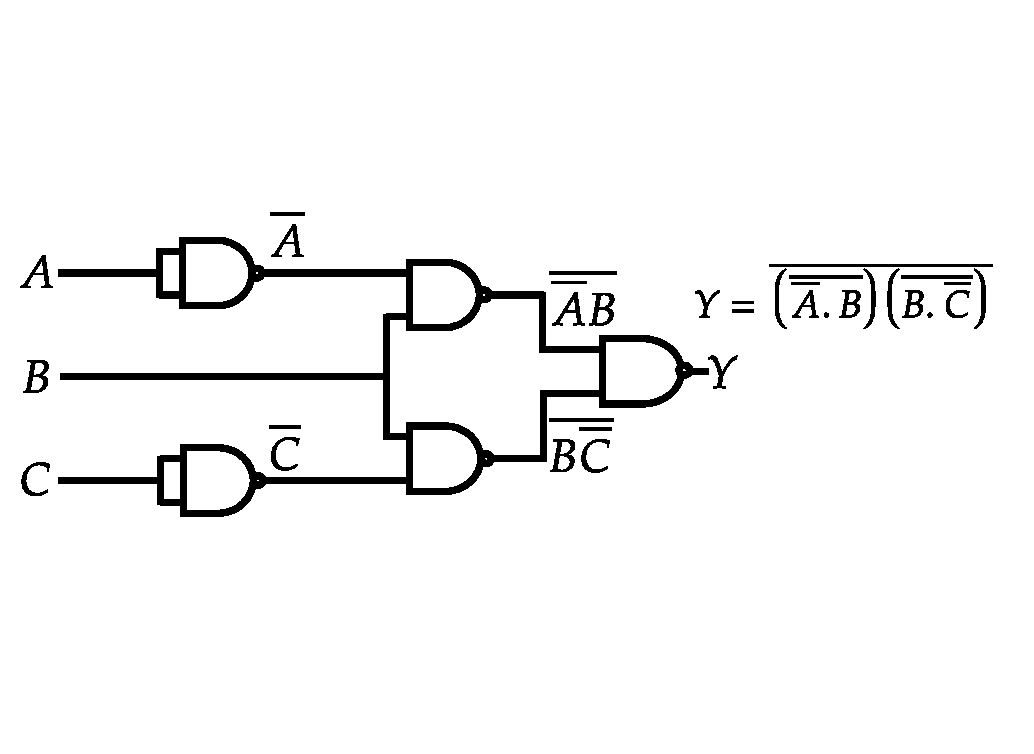
\includegraphics[height=7cm,width=10cm]{diagram-20210816(17)}
\end{figure}
\begin{align*}
Y&=\overline{(\overline{\bar{A}} B) \cdot(\overline{B . \bar{C}})}=\overline{(A+\bar{B})(\bar{B}+C)}
\end{align*}
So the correct answer is \textbf{Option (A)}
\end{answer}
	
	
	
	
	
	
	
	
	
	
	
	
	
	
\end{enumerate}